\subsubsection{Infiniton CITYJam Pro}
\label{apartado_patinetes}
\paragraph{Descripción general}

Estudiando las consideraciones descritas en el \refanexo{anexo_patienete eléctrico}, se ha optado de entre todos los modelos por la Infiniton CITYJam Pro \cite{infinitoncityjam}, mostrado en la \autoref{fig:Infinity CityJam}.

\begin{figure}[h]
    \centering
    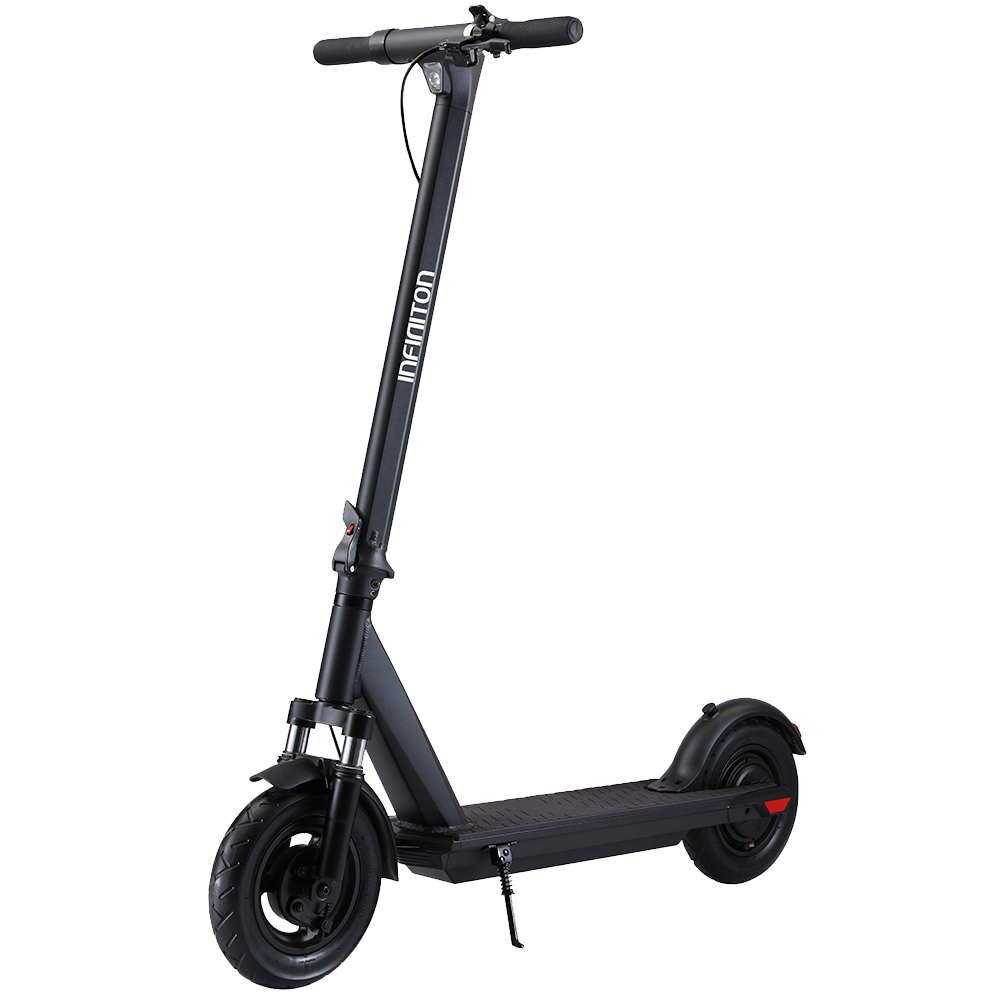
\includegraphics[scale = 0.2]{archivos/cityjam-pro-negro.jpg}
    \caption{Infiniton CITYJam Pro.}
    \label{fig:Infinity CityJam}
\end{figure}

Los motivos para elegir este modelo se fundamentan en su larga autonomía frente a los demás, y su capacidad en batería, permitiendo cargas más económicas y espaciadas en el tiempo. No se han tenido en consideración la inclinación del terreno o el peso máximo, dado que el rango de destino, terreno de la ciudad, y tipos de pedidos no suponen la  importancia necesaria.

La Infiniton CITYJam Pro tiene una autonomía de entre 40-45 \glssymbol{km} de distancia gracias a su batería de 350 \glssymbol{vatiohora}. Al igual que otros modelos en el mercado, cuenta con un sistema de recarga de energía cuando se frena, permitiendo prolongar la vida de cada carga.

Dispone de mucha estabilidad y durabilidad gracias al uso de acero resistente en su fabricación, junto con tres sistemas de frenos distintos y luces frontales y traseras para garantizar la seguridad del usuario.

La potencia que ofrece este modelo permite transportar cargas de hasta 100 \glssymbol{kg}, siendo suficiente para transportar al repartidor junto con el pedido.

\paragraph{Mantenimiento y robustez}

El patinete está fabricado con los materiales necesarios para soportar el día a día frente a un uso de ciudad. Además de ello, cuenta con un grado de protección IP54, controlado por la norma internacional CEI 60529 \cite{une60529}, capaz de soportar lluvia y polvo sin ningún tipo de problema.

El mantenimiento \cite{mantenimientopatinete} es más sencillo y económico comparado con un coche o una moto. Se recomienda emplear siempre piezas originales y no utilizar cargadores distintos al original. La limpieza del vehículo se puede realizar con ayuda de un trapo y cepillo, evitando el uso de mangueras de presión localizados en lavaderos de coches. 

Por otro lado, el modelo que estudiamos tiene ruedas de diez pulgadas, por lo que su durabilidad frente al desgaste va a ser alta. En caso de daño o fin de su vida útil, se pueden sustituir manualmente con recambios, sin necesidad de acudir a un taller especializado.

En referencia al sistema electrónico o la batería, se ha de evitar manipularlo, y en caso de avería llevarlo a un taller especializado. Las reparaciones dependen del daño y del taller al que se acuda, pero su precio no excede el de una avería de moto u otros tipos de vehículos.

Además de todo lo anterior, tal y como se indica en el \refanexo{anexo_precio_taller_combustible}, se incluye una cantidad fija de ahorro para caso de siniestro y sustitución de patinete.

\paragraph{Viabilidad económica}

Para ver si es aceptable el gasto hay que observar el gasto fijo que supone la adquisición del equipo al completo, y posteriormente el gasto anual entre mantenimiento, seguros y recargas. 

Todos los cálculos y estimaciones referentes a la viabilidad económica se pueden encontrar en la \autoref{tab: analisis_presupuestos_patienetes}, \refanexo{sub_anexo_calculos_patinete}, donde se muestran los presupuestos para ambos modelos de reparto estudiados en el estudio del reparto.

En el primer año, se han de tener en consideración el precio de mercado por unidad de los patinetes y el número total de patinetes que se van a comprar, según el \refanexo{anexo_calculos_sobre_vehiculos} son necesarios un total de 20 patinetes según la hipótesis de reparto de 5 \glssymbol{km} y 16 según la hipótesis de pedidos dobles. Además de esto, hay que añadir como gasto fijo inicial la adquisición del equipamiento, los cuales se enumeran en la \autoref{consideraciones_preliminares}, considerando en cada caso el número de empleados, o vehículos simultáneos en carretera que en este modelo serán 8 y 7, respectivamente.

Para los gastos anuales se debe comenzar con el coste de recarga del vehículo. Teniendo el precio de la luz, obtenido en el \refanexo{anexo_precio_taller_combustible} y el número de recargas semanales totales, junto con la capacidad de una batería, se obtiene el gasto semanal y anual relacionado con la recarga.

Los gastos relacionados con reparaciones o mantenimiento se han fijado en el \refanexo{anexo_precio_taller_combustible}, por lo que se asume un gasto mensual a cada uno. 

El coste por seguro fijado es de 35 \gls{euro}, lo cual se multiplicará directamente por el número de vehículos en posesión de manera mensual.

Teniendo todas las consideraciones anteriores descritas, se concluye finalmente el presupuesto necesario en el primer año y posteriores, siendo:

\begin{itemize}
    \item Presupuesto para el primer año del modelo de estudio 1 - 12.323,53 \gls{euro}
    \item Presupuesto anual del modelo de estudio 1 - 3.873,05 \gls{euro}
    \item Presupuesto para el primer año del modelo de estudio 2 - 9.926,05 \gls{euro}
    \item Presupuesto anual del modelo de estudio 2 - 3.096,81 \gls{euro}
\end{itemize}


\paragraph{Conclusiones modelo.}

Analizando los datos obtenidos, se llega a la conclusión que en cuestiones económicas, el patinete eléctrico es una de las opciones más baratas del mercado. A pesar de ser necesario una flota grande inicial para disponer siempre de un vehículo operativo, el coste sigue siendo menor que otras alternativas.

El coste energético es proporcional al precio de la electricidad, aunque comparado con la gasolina sigue siendo una alternativa eficiente y económica.

Los inconvenientes de este modelo de transporte son por un lado la seguridad del conductor, debido a lo vulnerable que es a los accidentes en carretera y condiciones meteorológicas, y por otro lado la cantidad necesaria de vehículos para garantizar el correcto funcionamiento del servicio, debido a que implica la posesión de las tomas de corriente suficientes para realizar múltiples cargas simultaneas.